\chapter{General setup of the hydrodynamic computation (Navier-Stokes equations)}

The general setup of the computation is only performed at the steering file
level.

The time data is provided by the two keywords \telkey{TIME STEP} (real, set at
1. by default) and \telkey{NUMBER OF TIME STEPS}. The first keyword sets the
period of time between two consecutive computational moments (but not
necessarily two outputs in the result file). The global duration of the
computation is provided through a number of time steps (keyword \telkey{NUMBER
OF TIME STEPS}, set at 1 by default) or a duration in seconds (keyword
\telkey{DURATION}, set at 0. by default). If both are given, \telemac{3D} follows
the instruction leading to the longest computation.

Both date and hour corresponding to the initial time of the computations can be
specified using the keywords \telkey{ORIGINAL DATE OF TIME}
(AAAA, MM, JJ format; default value = 1900; 1; 1) and \telkey{ORIGINAL
HOUR OF TIME} (HH, MM, SS format, default value = 0; 0; 0).
These two data are mandatory if using the tidal data bases.
They can be taken into account in programming by means of the \telfile{MARDAT}
and \telfile{MARTIM} variables.

The computation title is specified by the keyword \telkey{TITLE}.


\section{Mesh definition}

The three-dimensional mesh, consisting of prisms possibly cut into
tetrahedrons, is automatically constructed by \telemac{3D} from the
two-dimensional mesh. This construction is done in the subroutine
\telfile{CALCOT} from the information given by the subroutine defining the
initial conditions \telfile{CONDIM}.

The number of prisms is specified in the data file by means of the keyword
\telkey{NUMBER OF HORIZONTAL LEVELS} (default value = 2). That number of levels
is equivalent to the number of stacked prisms plus 1. Its minimum value is 2 (1
prism in the vertical direction).

\telemac{3D} uses a change of variables in order to freeze the mesh on a time
step (without such a change, the mesh dimensions $z$ would vary in
accordance with the free surface evolution). The frequently adopted change of
variables is the sigma transform which consists in shifting from the $z(x,y,t)$
co-ordinate to the $z^{*} (x,y)$ co-ordinate.
The user should enter the $z^{*}$ co-ordinates in the \telfile{CONDIM} subroutine.
The normalized co-ordinates will then range from 0 (the bottom) to 1 (the surface).

The numbering of levels is made according to upward vertical. Level 1 follows
the bottom and level $N$ corresponds to the free surface ($N$
being specified by the keyword \telkey{NUMBER OF HORIZONTAL LEVELS}).

The vertical mesh definition is based on the \telfile{TRANSF\_PLANE} table which
allows defining the behaviour of each level.

The keyword \telkey{MESH TRANSFORMATION} sets the kind of level distribution
along the vertical. The value 0 corresponds to a distribution directly defined
by the user in the \telfile{CALCOT} subroutine.

\begin{figure}[H]%
\begin{center}
%
  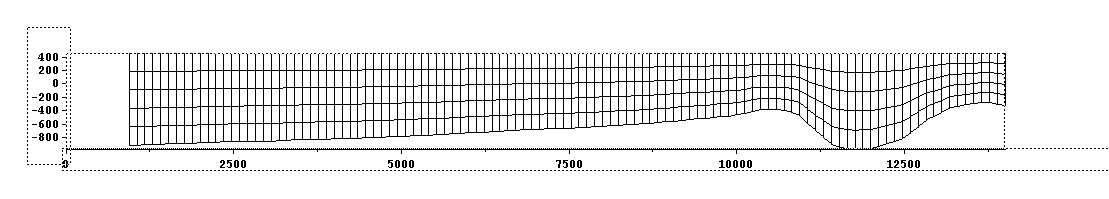
\includegraphics[width=\textwidth]{./graphics/mesh_transformation}
%
\end{center}
\caption
[Effect of the \telkey{MESH TRANSFORMATION}]
{Effect of the \telkey{MESH TRANSFORMATION} keyword -- Value 1: sigma.}
\label{fig:mesh_transf}
\end{figure}

The default value is 1 (Figure \ref{fig:mesh_transf}) and results in a
homogeneous distribution of levels in the vertical direction (classical sigma
transformation). The height of the levels varies depending on the water depth,
all planes can move (except for the bottom). In this case, no programming in
the \telfile{CONDIM} subroutine is required.

A value of 2 (Figure \ref{fig:mesh_transf2}) will allow the user to define the
distribution of levels (e.g. refinement near surface) while maintaining the
levels mobility (sigma transformation with given proportions). The latter
choice implies that the user will program his/her distribution in the
\telfile{CONDIM} subroutine to define the array \telfile{ZSTAR} that describes
the distribution of levels along the vertical as a percentage of the water depth.
Changes to make are:

\begin{itemize}
\item Specifying the variable \telfile{TRANSF\_PLANE} with a value of 2
for every level,

\item Specifying the level distribution along the vertical through the array
\telfile{ZSTAR} which describes the distribution along the vertical as a
percentage of the water depth (the values are between 0. and 1.).
\end{itemize}

For example (Figure \ref{fig:mesh_transf2}):

\begin{lstlisting}[language=TelFortran]
DO IPLAN = 1,NPLAN
  TRANSF_PLANE%I(IPLAN)=2
ENDDO

ZSTAR%R(1)=0.D0
ZSTAR%R(2)=0.02D0
ZSTAR%R(3)=0.1D0
ZSTAR%R(4)=0.4D0
ZSTAR%R(5)=0.8D0

\end{lstlisting}

\begin{figure}[H]%
\begin{center}
%
  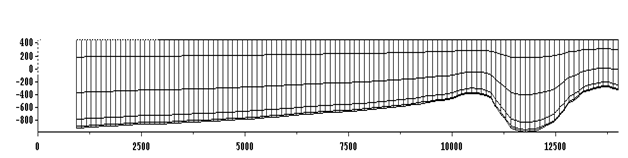
\includegraphics[width=\textwidth]{./graphics/mesh_transformation2}
%
\end{center}
\caption
[Effect of the \telkey{MESH TRANSFORMATION2}]
{Effect of the \telkey{MESH TRANSFORMATION} keyword -- Value 2: zstar.}
\label{fig:mesh_transf2}
\end{figure}

In order to better represent the densimetric stratification areas
(thermoclines, halocline and/or outfall), prescribing a maximum number of
horizontal "levels" (particularly those where the gradients are the highest) is
sometimes suitable. For that purpose, the user can select the value 3 for the
keyword \telkey{MESH TRANSFORMATION}. In this configuration, the user can
freely use the 3 types of level definition available in \telemac{3D} to create
the mesh along the vertical:

\begin{itemize}
\item Fixed levels at a given altitude (correspond to value 3 of the
\telfile{TRANSF\_PLANE} variable, the altitude is specified by the
\telfile{ZPLANE} variable),

\item Irregularly distributed movable levels between two fixed levels
(correspond to value 2 of the \telfile{TRANSF\_PLANE} variable,
the distribution is specified by the \telfile{ZSTAR} variable),

\item Evenly distributed movable levels between two fixed levels (correspond
to value 1 of the \telfile{TRANSF\_PLANE} variable).
\end{itemize}

This latter choice requires the user to make changes in the \telfile{CONDIM}
subroutine:

\begin{itemize}
\item Specifying the variable \telfile{TRANSF\_PLANE} at value 1, 2 or 3
for each level,

\item Specifying the level distribution along the vertical through the array
\telfile{ZSTAR} for levels of type 2,

\item Specifying the level altitude through the array \telfile{ZPLANE} 
for levels of type 3.
\end{itemize}

For example (Figure \ref{fig:mesh_transf3}):
\begin{lstlisting}[language=TelFortran]
DO IPLAN = 1,5
  TRANSF_PLANE%I(IPLAN)=2
ENDDO
ZSTAR%R(1)=0.D0
ZSTAR%R(2)=0.2D0
ZSTAR%R(3)=0.5D0
ZSTAR%R(4)=0.7D0
ZSTAR%R(5)=0.8D0

DO IPLAN = 7,NPLAN
 TRANSF_PLANE%I(IPLAN)=1
ENDDO

TRANSF_PLANE%I(6)=3
ZPLANE%R(6)=0.D0
\end{lstlisting}

\begin{figure}[H]%
\begin{center}
%
  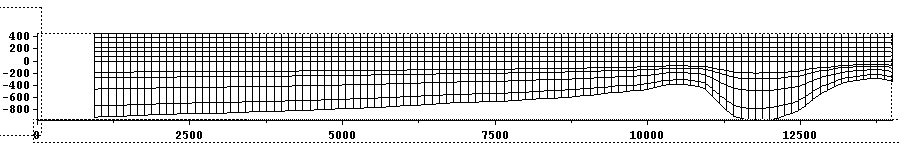
\includegraphics[width=\textwidth]{./graphics/mesh_transformation3}
%
\end{center}
\caption
[Effect of the \telkey{MESH TRANSFORMATION3}]
{Effect of the \telkey{MESH TRANSFORMATION} keyword -- Value 3: user defined.}
\label{fig:mesh_transf3}
\end{figure}

Various programming examples are provided as comments in the \telfile{CONDIM}
subroutine.

The triangular based prismatic elements can optionally be split into
tetrahedrons. This option is enabled using the \telkey{ELEMENT} keyword can
take the value 'PRISM' (default value) or 'TETRAHEDRON'.


\section{Prescribing the initial conditions}

The initial conditions aim at defining the model condition at the beginning of
the simulation.

In case of a continuing computation, the initial conditions are provided at one
time step in the result file of the previous computation (refer to section
\ref{sec:previousfile}).
The mandatory variables (at least the velocity components) when resuming
the computation should then have been stored into the file being used as
\telkey{PREVIOUS COMPUTATION FILE}.

Otherwise, the default initial condition is defined as follows:

\begin{itemize}
\item Free surface set to an elevation equal to 0,

\item Zero velocities,

\item Steady zero active and passive tracers.
\end{itemize}

If that initial condition is not suitable for a computation, then it should be
changed using keywords in the simple cases or through a programming as
described in the subsequent subsections.


\subsection{Prescription through keywords}

In all the cases, the kind of initial conditions is set by the keyword
\telkey{INITIAL CONDITIONS}. That keyword can have one of the following six
values:

\begin{itemize}
\item 'ZERO ELEVATION': Initializes the free surface elevation
to 0 (default value). The initial water depths are then computed from the
bottom depth,

\item 'CONSTANT ELEVATION': Initializes the free surface elevation to the
values as provided by the keyword \telkey{INITIAL ELEVATION}. The initial water
depths are then computed by getting the difference between the free surface
elevation and the bottom depth.  In those areas where the bottom depth exceeds
the initial elevation, the initial water depth is zero,

\item 'ZERO DEPTH': All the water depths are initialized with a zero value
(free surface coinciding with bottom). In other words, the whole domain is
"dry" at the beginning of the computation,

\item 'CONSTANT DEPTH': Initializes the water depths to the value as provided
by the keyword \telkey{INITIAL DEPTH},

\item `TPXO SATELLITE ALTIMETRY': The initial conditions are set using
information provided by the OSU harmonic constants database (TPXO for instance)
in the case of the use of this database for the imposition of maritime boundary
conditions (see subsection \ref{sec:tide}),

\item 'PARTICULAR' or 'SPECIAL': The initial conditions are defined as
programmed by the user in the \telfile{CONDIM} subroutine (refer to the next
subsection).
That procedure should be used whenever the initial conditions of the model do 
not correspond to one of above four cases.
\end{itemize}


\subsection{Prescribing particular initial conditions (Programming the \telfile{CONDIM} subroutine)}
\label{sec:prescr_IC}

The \telfile{CONDIM} subroutine should be programmed whenever the initial
conditions programmed by default are to be modified.

By default, the standard version of the \telfile{CONDIM} subroutine interrupts
the computation if the keyword \telkey{INITIAL CONDITIONS} is set to 'PARTICULAR'
without any actual amendment of the subroutine.

The \telfile{CONDIM} subroutine successively initializes the two-dimensional
variables, then the three-dimensional variables:

\begin{itemize}
\item The water depth,

\item The 3D component of velocities,

\item The active and passive tracers.
\end{itemize}

The user can quite freely fill that subroutine. For instance, he/she can
retrieve information in a formatted or binary file, using the corresponding
keywords.


\subsection{Resuming the computation}

telemac{3D} enables the user to resume a computation by taking as the initial
condition the last time step of a computation which was previously computed on
the same mesh, or possibly with a different number of levels. Thus, some
computational parameters such as the time step, some boundary conditions, the
turbulence model can be modified, or else a computation can be initiated once a
steady state is achieved.

The file to be retrieved shall then inevitably contain all the data required
for \telemac{3D}, i.e. not only the co-ordinates of the $X$, $Y$
and $Z$ computational points which it necessarily contains, but also the
3D velocities and the tracers.

If some variables do not appear in the \telkey{PREVIOUS COMPUTATION
FILE}, then they are automatically set to zero values.  A usual application
consists in using the result of a hydrodynamic computation in order to perform
a tracer transport computation. Generally, the \telkey{PREVIOUS COMPUTATION
FILE} does not include any result for the tracer.

To resume a computation, it is required to use two keywords into the steering
file.

The keyword \telkey{COMPUTATION CONTINUED} should be set to the YES value.

The keyword \telkey{PREVIOUS COMPUTATION FILE} should provide the name of the
file which will provide the initial conditions (default value = 0).

Optionally, the keyword \telkey{RECORD NUMBER FOR RESTART} can be used to
define the record number to read if it is not the last one (defined by a
default value set to 0).

\begin{WarningBlock}{Warning:}
The two-dimensional mesh on which the useful results have been computed should
be strictly identical to the mesh of the case to be handled.
\end{WarningBlock}

Resuming the computation usually leads to small differences in results
compared to the same calculation without interruption. This difference is
mainly due to the fact that the velocity advection is not treated properly at
the first time step, because this operation requires information from the
previous time step. To correct this, the user has a specific recovery procedure
to improve the accuracy of calculations, using double precision format SERAFIN
files:

\begin{itemize}
\item In the first computation, the keyword \telkey{RESTART MODE} is set to
YES, which generates a specific file containing the full information only of
the last time step of the simulation (in particular information on the
advection field of the last time step). The name of this file is specified
using the keyword \telkey{RESTART FILE},

\item In the second computation, this specific file must be used as
\telkey{PREVIOUS COMPUTATION FILE} specifying the \telkey{PREVIOUS COMPUTATION
FILE FORMAT} is 'SERAFIND' (SERAFIN double precision). In this case, the
keyword \telkey{RECORD NUMBER FOR RESTART} cannot be used because the recovery
file only contains the last time step of the simulation.
\end{itemize}

However, it has to be mentioned that even if it is not advisable, the creation
of specific restart file can be done not only SERAFIND format, but also with
any other available format in the TELEMAC system, especially in single
precision. In this case, the keyword \telkey{RESTART FILE FORMAT} (by default
set at 'SERAFIND') must be set to the proper value.

A particular aspect of the resuming technique of computation is the value of
the start time of the second simulation. By default, the start time of the
second calculation is equal to the value of the last time step of restart file.
This can be changed by using the logical keyword \telkey{INITIAL TIME SET TO
ZERO} if the user wants to start from zero (default value is NO).

It is also possible to resume a computation from a 2D results file. This is
generally useful in river hydraulic offering the possibility to initialise the
model in 2D before shifting to 3D simulation. In this case, the horizontal
velocities are considered as constant on the vertical and equal to the 2D
velocities and the vertical velocities are initialised to zero. This
possibility is activated using the \telkey{2D CONTINUATION} logical keyword
(default value = NO). The 2D results file must be given using \telkey{FILE FOR
2D CONTINUATION}. The keyword \telkey{FILE FOR 2D CONTINUATION FORMAT} gives
the format of the file and can takes the following values: `SERAFIN ' (default
value), `SERAFIND' and `MED'.


\section{Prescribing the boundary conditions}
\label{sec:prescr_BC}

The boundary conditions are handled through types of conditions which are
related to the computational variables. The combination of these types (from a
list of possible choices) describes whether the boundary is liquid or solid and
how it should be processed.

In \telemac{3D}, the water depth $H$, the horizontal velocities $U$
and $V$ and the tracers are the only variables which necessarily involve
defining their type of boundary conditions. Those types of boundary conditions
applicable to the vertical velocity and the $k$ and $\epsilon$ functions
are managed by \telemac{3D} by the user directly in the FORTRAN source files of
\telemac{3D} and therefore do not have a type. If the computation takes tracers
into account, then a single type (common to all the tracers) should also be
defined for a given boundary.

Once all the types of the boundary are defined, the user should enter the
related values for the computational variables (at least $H$, $U$ and $V$).

For example, the user may want to set the sea level and leave the velocity
field free (e.g. the tide case). The type of boundary will be: "prescribed
depth and free velocity". The values required for that type are only water
depth at every instant at that boundary. The values of velocities (if they are
entered) are not taken into account for that boundary.

Thus, for each \telemac{3D} boundary, the computational variables (at least
$H$, $U$ and $V$) are necessarily associated with one type
and each type may be associated with one value (either used or not).

The maximum number of boundaries is set to 30 by default but it can be changed
by the user with the keyword \telkey{MAXIMUM NUMBER OF BOUNDARIES}.
This avoids changing the previously hardcoded values (until version 7.0),
which required recompiling the whole package.

After such a description of what is a boundary in \telemac{3D}, we will describe
the types, then the related values.

\subsection{The boundaries in \telemac{3D}}

Water depth is the only two-dimensional variable computed. Its processing at
the boundaries is like that being performed by \telemac{2D}. The boundary points
to be handled are those of the two-dimensional mesh (refer to Figure
\ref{fig:bnd}).

For the other variables (velocities and tracers), the boundary conditions
should be handled over all the boundaries of the three-dimensional mesh which
includes:

\begin{itemize}
\item The lateral boundary points (vertical column points linked to the
boundaries of the two-dimensional mesh), whether it is a liquid or solid
boundary,

\item The points belonging either to the free surface or the bottom.
\end{itemize}

\begin{figure}[H]%
\begin{center}
%
  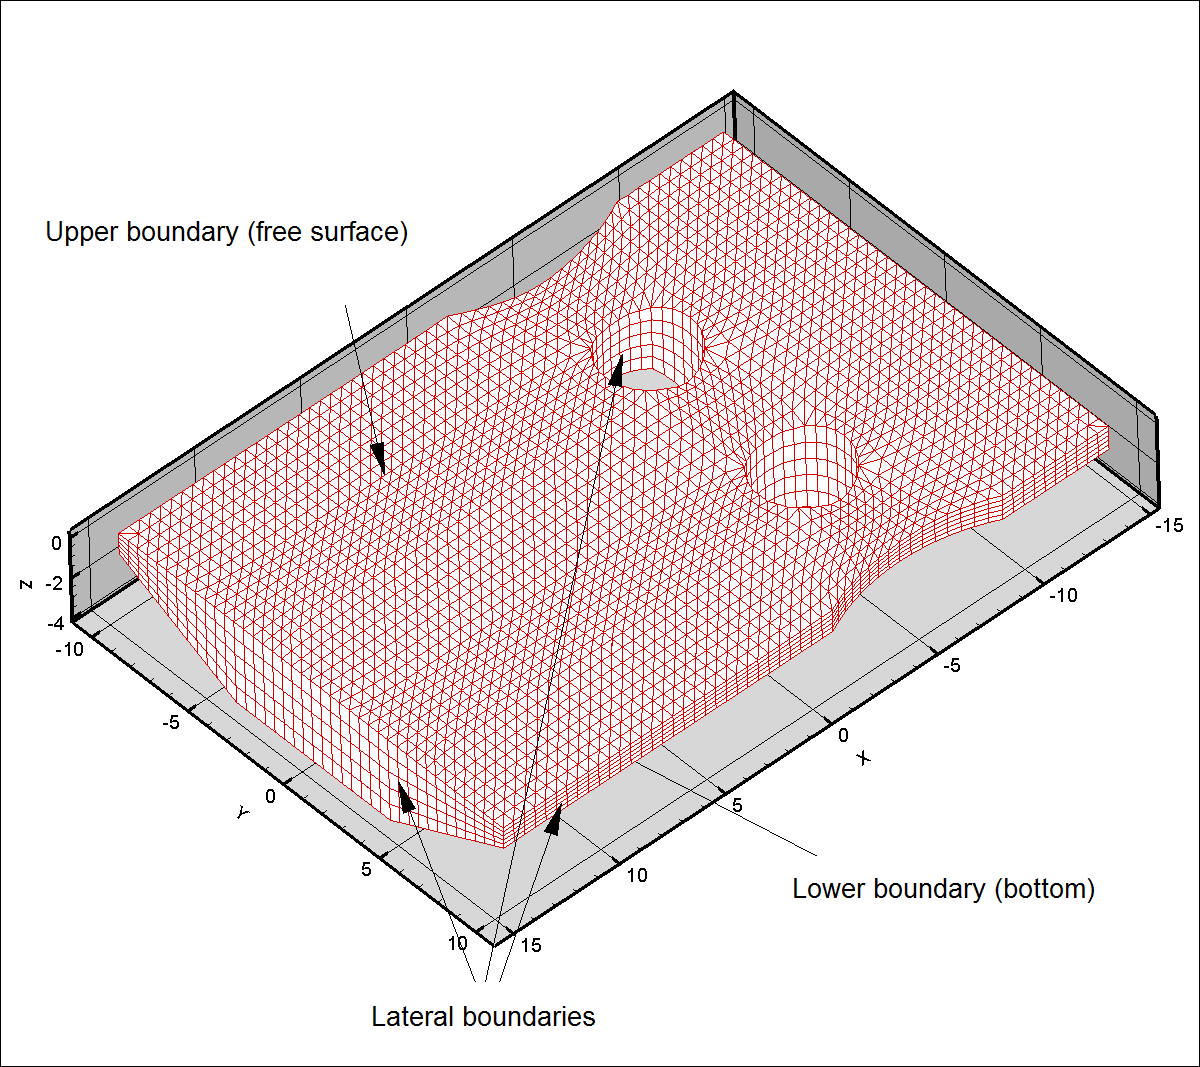
\includegraphics[width=0.7\textwidth]{./graphics/bnd}
%
\end{center}
\caption
[Boudnaries in \telemac{3D}]
{The various boundaries in \telemac{3D} (bridge piers case study).}
\label{fig:bnd}
\end{figure}

By default, \telemac{3D} automatically handles all the surface and bottom points
which do not belong to the side walls. The user, however, can modify them. This
can be done by modifying the FORTRAN sources.

All the remaining points (on the lateral boundaries) are linked to the
two-dimensional mesh boundaries at each horizontal level. Thus, they will be
processed in a similar fashion as in \telemac{2D}. The number of required data,
however, increases so much that a full external handling (either through the
steering file or the boundary conditions file) would become excessively
complex. That is why the range of options offered to the user for dealing with
these boundary conditions is narrower than in \telemac{2D} and definitely implies
programming the sources of the user-available software. The next following
subsections describe the way the boundary nodes are handled.


\subsection{The boundary-related types}

The boundary condition type for $H$, $U$, $V$ and $T$ of the edge points is
read in the boundary conditions file. It can be either modified or directly
defined by the user in the \telfile{LIMI3D} subroutine.

The various types of boundary conditions can be combined in order to prescribe
the conditions of different physical kinds (liquid inflow or outflow in
supercritical conditions, open sea, wall, etc.). Some combinations, however,
are not physical (refer to subsection \ref{sec:descr_bnd} hereinafter).

Some boundary conditions are applicable to such facts as friction at the walls
or wall impermeability. However, the wall definition is ambiguous if one only
retains a definition of point wise boundary conditions. The following
convention is then observed in order to determine the nature of a segment lying
between two different kinds of points: a liquid segment is a segment linking
two liquid-types points. Thus, under that convention, the connecting point
between the shore and the marine boundary (or between the river and the bank)
is preferably of the liquid type. Therefore, liquid + solid = solid

Any sequential arrangement of the boundary types may exist along an outline
(for instance, one may have a liquid boundary with a prescribed depth followed
by a liquid boundaryliquid boundary with a prescribed velocity). The only
condition to be met is that a boundary should consist of at least two points
(it is a computational requirement, a number of at least four points being
highly advisable from a physical point of view).


\subsection{Description of the various types}
\label{sec:descr_bnd}

The type of boundary condition at a given point is provided, in the boundary
conditions file, in the form of four integers which are referred to as
\telfile{LIHBOR}, \telfile{LIUBOR}, \telfile{LIVBOR} and \telfile{LITBOR},
with values which can range from 0 to 6.

The available options are as follows:

\begin{itemize}
\item Depth condition:

\begin{itemize}
\item Prescribed depth liquid boundary: \telfile{LIHBOR}=5,

\item Free depth liquid boundary: \telfile{LIHBOR}=4,

\item Solid boundary (wall): \telfile{LIHBOR}=2.
\end{itemize}
\end{itemize}

It is noteworthy that a depth/rate law is considered as a prescribed depth
condition. The flow rate value should then explicitly be computed, according to
the water depth, by programming the Q3 subroutine.

\begin{itemize}
\item Rate or velocity condition:

\begin{itemize}
\item Prescribed flow rate liquid boundary: \telfile{LIUBOR/LIVBOR}=5,

\item Prescribed velocity liquid boundary: \telfile{LIUBOR/LIVBOR}=6,

\item Free velocity liquid boundary: \telfile{LIUBOR/LIVBOR}=4,

\item Solid boundary with sliding or friction: \telfile{LIUBOR/LIVBOR}=2,

\item Solid boundary with one or two zero velocity components: \telfile{LIUBOR} and/or
\telfile{LIVBOR}=0.
\end{itemize}

\item Tracer condition:

\begin{itemize}
\item Prescribed tracer liquid boundary: \telfile{LITBOR}=5,

\item Free tracer liquid boundary: \telfile{LITBOR}=4,

\item Solid boundary (wall): \telfile{LITBOR}=2.
\end{itemize}
\end{itemize}


\subsection{The boundary conditions file}
\label{sec:bndfile}
That file is provided as standard by MATISSE, Janet, Blue Kenue or \stbtel, but
it can be created or amended by means of FUDAA-PREPRO or a text editor. Each
line of that file is dedicated to one point at the two-dimensional mesh
boundary. The boundary point numbering is the same as that of the file lines,
it first describes the domain outline in the counter clockwise direction, then
the islands in the opposite direction.

The convention being observed in TELEMAC implies that the first liquid boundary
is that which is defined, within the boundary conditions file, by the first two
liquid-typed consecutive numbers. In the example below (channel case study),
the first liquid boundary is defined by the nodes 42-47 (edge numbering) and
corresponds to a prescribed depth (codes 5 4 4 at the beginning of lines). The
second boundary begins at number 76 and ends at number 1 and corresponds to a
prescribed rate (codes 4 5 5).

\begin{lstlisting}[language=bash]
 4 5 5  0.000  0.000  0.000  0.0   2  0.000  0.000  0.000      1     1
 2 2 2  0.000  0.000  0.000  0.0   2  0.000  0.000  0.000      5     2
 2 2 2  0.000  0.000  0.000  0.0   2  0.000  0.000  0.000      6     3
...
 2 2 2  0.000  0.000  0.000  0.0   2  0.000  0.000  0.000     44    41
 5 4 4  0.000  0.000  0.000  0.0   2  0.000  0.000  0.000      2    42
 5 4 4  0.000  0.000  0.000  0.0   2  0.000  0.000  0.000     45    43
 5 4 4  0.000  0.000  0.000  0.0   2  0.000  0.000  0.000     86    44
...
 5 4 4  0.000  0.000  0.000  0.0   2  0.000  0.000  0.000      3    47
 2 2 2  0.000  0.000  0.000  0.0   2  0.000  0.000  0.000     87    48
...
 2 2 2  0.000  0.000  0.000  0.0   2  0.000  0.000  0.000     73    74
 2 2 2  0.000  0.000  0.000  0.0   2  0.000  0.000  0.000     74    75
 4 5 5  0.000  0.000  0.000  0.0   2  0.000  0.000  0.000      4    76
 4 5 5  0.000  0.000  0.000  0.0   2  0.000  0.000  0.000     88    77
...
 4 5 5  0.000  0.000  0.000  0.0   2  0.000  0.000  0.000     89    85
\end{lstlisting}

For each point, and each line in the boundary conditions file, the following
values are entered:

\telfile{LIHBOR, LIUBOR, LIVBOR, HBOR, UBOR, VBOR, AUBOR, LITBOR, TBOR, ATBOR,
BTBOR, N, K}

\begin{itemize}
\item  \telfile{LIHBOR, LIUBOR, LIVBOR} and \telfile{LITBOR} are boundary-typed
integers for each of the variables.

\item \telfile{HBOR} (real) denotes the prescribed depth value when the
\telfile{LIHBOR} value is set to 5,

\item \telfile{UBOR} (real) denotes the prescribed $U$ velocity value when
the \telfile{LIUBOR} value is set to 6,

\item \telfile{VBOR} (real) denotes the prescribed $V$ velocity value when
the \telfile{LIVBOR} value is set to 6,

\item \telfile{AUBOR} denotes the value of the boundary friction coefficient when
the \telfile{LIUBOR} or \telfile{LIVBOR} value is set to 2.
The friction law is then written as:
%TODO: Space between equations
\begin{align}
\upsilon_{T} \frac{dU}{dn} = AUBOR \times U {\rm and/or }
\upsilon_{T} \frac{dV}{dn} = AUBOR \times V
\end{align}
\end{itemize}
The \telfile{AUBOR} coefficient is applicable to the segment included between
the edge point being considered and the next point (in the counter clockwise
direction for the outside outline and in the clockwise direction for the islands).
By default, the \telfile{AUBOR} value is 0.
A friction corresponds to a negative value.
With the $k$-$\epsilon$ model, the value of \telfile{AUBOR} is automatically
computed by \telemac{3D}, the indications in the boundary conditions file will
then be ignored.

\begin{itemize}
\item \telfile{TBOR} (real) denotes the prescribed tracer value when the
\telfile{LITBOR} value is set to 5,

\item \telfile{ATBOR} et \telfile{BTBOR} denote the coefficient values of the
flux law which is written as:
\begin{align}
\upsilon _{T} \frac{dT}{dn} = ATBOR \times T + BTBOR
\end{align}
\end{itemize}
The \telfile{ATBOR} and \telfile{BTBOR} coefficients are applicable to the
segment included between the edge point considered and the next point
(in the counter clockwise direction for the outside outline and in the
clockwise direction for the islands).

\begin{itemize}
\item \telfile{N} denotes the edge point global number,

\item \telfile{K} denotes the point number in the edge point numbering. This
number also represents a node colour (as an integer). This number named
\telfile{BOUNDARY\_COLOR},
can be used in parallel simulations to simplify the implementation of specific
cases. Without particular modification, this value is the rank of the border
point in the global numbering.
For example, a test like \telfile{IF (I.EQ.144) THEN} can be replaced by
\telfile{IF (BOUNDARY\_COLOUR\%I(I).EQ.144) THEN} which is compatible with
the parallel mode. However, this only concerns the 2D mesh (Table
\telfile{BOUNDARY\_COLOUR} is only given for level 1).
Be careful not to modify the last column of the boundary conditions file
that contains this \telfile{BOUNDARY\_COLOUR} table,
when using tidal harmonic constants databases (cf. [6]).
\end{itemize}

As regards the horizontal velocities, all the points in one water column will
have the same type of boundary condition defined by \telfile{LIUBOR} or
\telfile{LIVBOR}.
That principle is intrinsic to the \telemac{3D} formulation. Prescribing a
different type of boundary condition in the vertical direction (e.g. for a
subterranean stream) may, indeed, induce severe inconsistencies with the
hydrostaticity hypothesis and generate, for instance, unrealistic vertical
velocities. It is then advisable that the user will follow that principle.
Nonetheless, the boundary condition type in the vertical direction can be
altered through direct programming in the \telfile{LIMI3D} subroutine.

The so-called \telfile{LIHBOR}, \telfile{LIUBOR} and \telfile{LIVBOR} integers
(which define the boundary type) can assume a value ranging from 0 to 6.
The available options are as follows:

\begin{itemize}
\item Depth-related condition:

\begin{itemize}
\item Prescribed depth liquid boundary: \telfile{LIHBOR=5},

\item Free depth liquid boundary: \telfile{LIHBOR=4},

\item Solid boundary (wall): \telfile{LIHBOR=2},
\end{itemize}

\item Velocity-related condition:

\item Prescribed velocity liquid boundary: \telfile{LIUBOR/LIVBOR=6},

\item Prescribed rate liquid boundary: \telfile{LIUBOR/LIVBOR=5},

\item Free velocity liquid boundary: \telfile{LIUBOR/LIVBOR=4},

\item Solid boundary with sliding or friction: \telfile{LIUBOR/LIVBOR=2},

\item Solid boundary with one or two zero velocity components: \telfile{LIUBOR} and/or
\telfile{LIVBOR=0}.
\end{itemize}

The boundary conditions of physical nature are defined by the relationship
among the types of variables. In most cases, the boundary type can be set by a
mesh generator (e.g. MATISSE or Janet) in the TELEMAC chain. The table
below summarizes the physical relationship among the boundary types.


\begin{tabular}{|p{0.5in}|p{0.5in}|p{0.5in}|p{0.5in}|p{2.0in}|} \hline
LIHBOR & LIUBOR & LIVBOR & LITBOR &  \\ \hline
2 & 2 & 2 & 2 & Solid wall. \\ \hline
2 & 0 & 2 & 2 & Solid wall with zero $U$. \\ \hline
2 & 2 & 0 & 2 & Solid wall with zero $V$. \\ \hline
2 & 0 & 0 & 2 & Solid wall with zero $U$ and $V$. \\ \hline
4 & 4 & 4 & 4 & Free $H$, free velocities, free $T$. \\ \hline
5 & 4 & 4 & 4 & Prescribed $H$, free velocities, free $T$. \\ \hline
5 & 4 & 0 & 4 & Prescribed $H$, free $U$, zero $V$, free $T$. \\ \hline
5 & 0 & 4 & 4 & Prescribed $H$, zero $U$, free $V$, free $T$. \\ \hline
1 & 1 & 1 & 4 & Incident wave, free tracer. \\ \hline
4 & 5 & 5 & 5 & Free $H$, prescribed $Q$, prescribed $T$. \\ \hline
4 & 5 & 0 & 5 & Free $H$, prescribed $Q$ with zero $V$, prescribed $T$. \\ \hline
4 & 0 & 5 & 5 & Free $H$, prescribed $Q$ with zero $U$, prescribed $T$. \\ \hline
4 & 6 & 6 & 5 & Free $H$, prescribed velocities, prescribed $T$.
\\ \hline
5 & 5 & 5 & 5 & Prescribed $H$ and $Q$, prescribed $T$. \\ \hline
5 & 6 & 6 & 5 & Prescribed $H$ and velocities, prescribed $T$. \\
\hline
\end{tabular}


\subsection{Programming the boundary conditions type}

The \telfile{LIMI3D} subroutine can be programmed to handle specific boundary
conditions, for the edge points as well as the surface and bottom points.

That subroutine is called upon each time step. Therefore, it can be used to
change the boundary condition type in time, if required.


\subsection{Prescribing values through keywords}

In most simple cases, the boundary conditions will be prescribed by means of
keywords. However, if the values to be prescribed are variable in time, it is
necessary to program the adequate functions or to use the liquid boundaries
file.

The appropriate keywords to prescribe the boundary values are as follows:

\begin{itemize}
\item \telkey{PRESCRIBED ELEVATIONS}: provided to set the
elevation value of a prescribed height liquid boundary. It is an array which
can contain up to 100 reals, and therefore up to 100 boundaries of that kind
can be handled. The values defined by that keyword overwrite the depth values
read from the boundary conditions file,

\begin{WarningBlock}{Warning:}
The free surface level is set with this keyword, whereas the water depth is set
in the boundary conditions file.
\end{WarningBlock}

\item \telkey{PRESCRIBED FLOWRATES}: provided to set the flow rate value of a
prescribed flow at a liquid boundary. It is an array which can contain up to
100 reals, and therefore up 100 boundaries of that kind can be handled. A
positive value corresponds to a domain inflow rate. The values defined by that
keyword overwrite the velocity values read from the boundary conditions file,

\item \telkey{PRESCRIBED VELOCITIES}: provided to set the velocity value of a
prescribed velocity liquid boundary. The scalar value is the wall normal
velocity. A positive value corresponds to a domain inflow. It is an array which
can contain up to 100 reals, and therefore up 100 boundaries of that kind can
be handled. The values defined by that keyword overwrite the values read from
the boundary conditions file.
\end{itemize}

In addition, several simple rules should be observed:

The boundary type as specified in the boundary conditions files should
obviously be in accordance with the keywords in the steering file (do not
insert the keyword \telkey{PRESCRIBED FLOWRATES} if there are no boundary
points the \telfile{LIUBOR} and \telfile{LIVBOR} of which are set to
5). The keyword, however, is ignored if no type matches it.

For each keyword, the number of specified values should be equal to the whole
number of liquid boundaries, whatever their types may be. When a boundary is
inconsistent with the keyword, then the specified value is ignored (a 0.0 value
or, on the contrary, a very high value such as 999.0 may be systematically
inserted).

For example, in the channel test case, the first boundary (downstream boundary)
is of prescribed level type whereas the second one (upstream boundary) is of
prescribed flow rate type. The steering file contains a sequence of the
following type:

\begin{lstlisting}[language=TelemacCas]
PRESCRIBED ELEVATIONS = 0.5, 0.0
PRESCRIBED FLOWRATES  = 0.0, 50.0
\end{lstlisting}

\subsection{Boundary condition on the bottom}

By default, the boundary condition on the bottom is an impermeable slip
boundary (Neumann condition of the same type as vertical conditions).

However, bottom velocities can be set to zero by using value 2 of the keyword
\telkey{BOUNDARY CONDITION ON THE BOTTOM} (Default value of 1 correspond to a
slip condition). This option is valid only if the vertical mesh is refined at
bottom level.

Since version 7.1, it is possible to prescribe a flux on the bed in TELEMAC-3D
(e.g.: a flow rate on several liquid boundaries placed on the bed).
To do so, it is necessary to define the imposed flow rates using the keywords
\telkey{OPEN BOUNDARY CONDITIONS ON THE BED} set to YES (default value = NO)
and \telkey{PRESCRIBED FLOWRATES ON THE BED} with values following the same
structure as for other prescribed flow rates in the TELEMAC-MASCARET system.
It should be a list of numbers separated by a semi-colon, one number per
liquid boundary on the bed must be given.
The maximum number of boundaries on the bed is set to 30 by default
but it can be changed by the user with the keyword \telkey{MAXIMUM NUMBER OF
BOUNDARIES ON THE BED}.
At the moment, the \telkey{BOUNDARY CONDITIONS FILE} only deals with horizontal
boundaries, therefore the user has to define the liquid boundary on the bed by hand.
This can be done by modifying the subroutine LIMI3D in the \telkey{FORTRAN FILE}.
For example to add a circular boundary of radius 5~m centred around coordinate
(2~000, 2~000)~m, the following modifications can be done:
\begin{lstlisting}[language=TelFortran]
...
!     BOUNDARY CONDITIONS ON VELOCITIES
!     *********************************
!
!     BOTTOM
!     ======
!
!     DEFAULT: IMPERMEABILITY AND LOG LAW (SEE ALSO BORD3D)
!
      IF(BC_BOTTOM.EQ.1) THEN
!
        DO IPOIN2 = 1,NPOIN2
          LIUBOF%I(IPOIN2) = KLOG
          LIVBOF%I(IPOIN2) = KLOG
          LIWBOF%I(IPOIN2) = KLOG
!         USEFUL ? SHOULD NOT BE USED ANYWAY
          UBORF%R(IPOIN2)  = 0.D0
          VBORF%R(IPOIN2)  = 0.D0
          WBORF%R(IPOIN2)  = 0.D0
          IF(SQRT((X(IPOIN2)-2000.D0)**2
     &           +(Y(IPOIN2)-2000.D0)**2)
     &       .LE.50.D0) THEN
            !5: IMPOSED FLOW RATE
            LIUBOF%I(IPOIN2) = 5
            LIVBOF%I(IPOIN2) = 5
            LIWBOF%I(IPOIN2) = 5
            NLIQBED%I(IPOIN2) = 1
            WRITE(LU,*) '========================'
            WRITE(LU,*) 'FOR POINT ',IPOIN2
            WRITE(LU,*) 'BEDFLO',BEDFLO(1)
          ENDIF
        ENDDO
!
...
\end{lstlisting}

In this example, it should be noted that \telfile{NLIQBED\%I(IPOIN2)} = 1
defines the position for the first liquid boundary defined in the steering file.
This is all that needs to be defined by the user to deal with fluxes on the bed.
However, in version 7.1, only constant velocity profile is available.
It should also be noted that it has not been possible to prescribe a tracer
or turbulence yet.

\subsection{Using the liquid boundaries file}
\label{sec:liqbnd}
In case of time variable values, which are nonetheless constant in space along
the relevant liquid boundary, the prescription can be made using the liquid
boundaries file (as an alternative to programming).

It is a user-edited text file the name of which should be given by the keyword
\telkey{LIQUID BOUNDARIES FILE}. That file has the
following format:

\begin{itemize}
\item The optional line(s) begin(s) with the sign $\#$ (1st character on the
line) will be treated as comments,

\item It should contain a header line beginning with \telfile{T} for identifying
the supplied time dependent value(s) within that file. The identification is
performed through mnemonic means which are identical to the variable names:
\telfile{Q} for the flow rate, \telfile{SL} for the level, \telfile{U} and
\telfile{V} for the velocities and \telfile{TR} for the
tracer. These characters are directly followed by an integer in between
brackets which is used to specify the current boundary. That line is
necessarily followed by another line indicating the unit of the variables
(lines of comments can be inserted, but the line of units should be present).
The units are given for information only and \telemac{3D} does not handle the
conversion of units (thus, the user has to enter the values using the standard
unit),

\item The values to be prescribed are provided through a sequence of lines the
format of which should be consistent with the identification line. The time
value should be increasing and the last time value supplied should be higher
than or equal to the value of the last time step, otherwise the computation is
suddenly interrupted.
\end{itemize}

Upon the retrieval of that file, \telemac{3D} performs a linear interpolation in
order to compute the value prescribed at a particular time step. The value
which is actually prescribed by the code is printed on the check listing.

An example of a liquid boundaries file is given below.

\begin{lstlisting}[language=bash]
#  Example of liquid boundaries file
#  2 boundaries are managed
#
T Q(1) SL(2)
s m3/s m
0. 0. 135.0
25. 15. 135.2
100. 20. 136.
500. 20. 136.
\end{lstlisting}

In that example, the flow rate is prescribed at the first boundary and the free
surface is prescribed at the second boundary.


\subsection{Prescribing values through programming}

Still in the case of time variable values that are constant in time along the
liquid boundary processed, the prescription can be made simply by programming
particular functions:

\begin{itemize}
\item \telfile{VIT3} function for prescribing a velocity,

\item \telfile{Q3} function for prescribing a flow rate,

\item \telfile{SL3} function for prescribing an elevation.
\end{itemize}

Functions \telfile{Q3, VIT3} and \telfile{SL3} are similarly programmed.
In each case, the user knows the time, the boundary rank (e.g. to determine
whether the first or the second prescribed flow rate boundary is processed).
By default, the functions prescribe values that are read from the boundary
conditions file or provided by the keywords.

For instance, the body of function \telfile{Q3} used to prescribe a flow rate
ramp for the first 1,000 seconds from 0 to 400~m${}^{3}$/s can take such a form as:

\begin{lstlisting}[language=TelFortran]
IF (AT.LT.1000.D0) THEN
  Q3 = 400.D0 * AT/1000.D0
ELSE
  Q3 = 400.D0
ENDIF
\end{lstlisting}

Or

\begin{lstlisting}[language=TelFortran]
Q3 = 400.D0 * MIN(1.D0,AT/1000.D0)
\end{lstlisting}

\subsection{Stage-discharge curves}
\label{sec:discharge}
\telemac{3D} allows managing liquid boundaries for which the prescribed water
elevation value is a function of local flow rate. This situation is encountered
particularly in river hydraulics.

First, it is necessary to specify which boundaries are concerned with the
keyword \telkey{STAGE-DISCHARGE CURVES}. This keyword provides an integer value
for each boundary. This value can be:

\begin{itemize}
\item 0: no stage-discharge curves (default),

\item 1: elevation as a function of local flow rate.
\end{itemize}

The keyword \telkey{STAGE-DISCHARGE CURVES FILE} provides the name of the text
file containing information about the curves. An example is shown below:

\begin{lstlisting}[language=bash]
#
#  STAGE-DISCHARGE CURVE BOUNDARY 1
#
Q(1)      Z(1)
m3/s      m
61.       0.
62.       0.1
63.       0.2
#
#  STAGE-DISCHARGE CURVE BOUNDARY 2
#
Z(2)      Q(2)
m         m3/s
10.       1.
20.       2.
30.       3.
40.       4.
50.       5.
\end{lstlisting}

The order of curves has no significance. The column order can be reversed, as
is the case for the second boundary in the example.
Lines beginning with \telfile{\#} are comments.
The lines defining the units are mandatory but the units are not checked.
The number of points of each curve is completely free and need not be
the same for each curve.

Warning: at initial conditions, the flow at the exit can be null. The initial
level must correspond to that of the calibration curve otherwise a sudden
change is imposed. To avoid extreme situations, the curve should be limited to
a certain level of flow rate. In the example of boundary 1 above, the flow
rates below 61~m${}^{3}$/s generate a water elevation of 0~m above the flow of
63~m${}^{3}$/s to produce an elevation equal to 0.2~m.

\subsection{Prescribing complex values}

If the values to be prescribed vary in both space and time, then a programming
in the \telfile{BORD3D} subroutine becomes necessary, since that subroutine can
be used to prescribe the values in a node wise way.

That subroutine describes all the liquid boundaries (loop on \telfile{NPTFR2}).
For each boundary point, it determines the boundary type in order to prescribe
the adequate value (velocity, elevation or flow rate).
\telfile{BORD3D} programming to prescribe a flow rate, however, hardly makes
any sense, since the flow rate value is generally known for the whole boundary
rather than on each boundary segment.

If a prescribed flow rate inlet is surrounded by walls with an adherence, then
the corner velocities are cancelled.

Note that, the \telfile{BORD3D} subroutine also makes it possible to prescribe
the complex boundary values of the tracers.

\subsection{Prescribing a profile}


\paragraph{Horizontal profile}

When processing a prescribed flow rate or prescribed velocity boundary, the
user has the keyword \telkey{VELOCITY PROFILES} to specify which "horizontal"
velocity profile should be prescribed by \telemac{3D}. The following options are
possible:

\begin{itemize}
\item 1: The profile is normal and homogeneous along the boundary (default
option),

\item 2: The values of $U$ and $V$ are read from the boundary
conditions file (\telfile{UBOR} and \telfile{VBOR} values).
In case of a prescribed flow rate, these values are multiplied by a constant
in order to get the desirable flow rate,

\item 3: The velocity vector is normal to the boundary and its norm is read
from the boundary conditions file as the \telfile{UBOR} value. In case of a
prescribed flow rate, that value is multiplied by a constant in order to get
the desirable flow rate,

\item 4: The velocity vector is normal to the boundary and its norm is
proportional to the square root of the water depth,

\item 5: The velocity vector is normal to the boundary and its norm is
proportional to the square root of a virtual water depth computed from lowest
point of the free surface on the boundary.
\end{itemize}

\paragraph{ Vertical profile}

When processing a prescribed flow rate or prescribed velocity boundary, the
user has the keyword \telkey{VELOCITY VERTICAL PROFILES} to specify which
"vertical" velocity profile should be prescribed by \telemac{3D}. The options for
that keyword are:

\begin{itemize}
\item 0: programmed by the user,

\item 1: constant (default value for all the liquid boundaries),

\item 2: logarithmic.
\end{itemize}

The user programming is done within the \telfile{VEL\_PROF\_Z} subroutine.

Activating the keyword \telkey{DYNAMIC BOUNDARY CONDITION} (default value =
FALSE) also enables to prescribe a velocity at the free surface coherent with
the dynamic boundary condition.

\subsection{Thompson conditions}

In some cases, not all the necessary information concerning the boundary
conditions is available. This is usual for coastal domains where only the
values of the sea level on several points are known. This kind of model is
referred to as an ``under-constrained'' model.

To solve this problem, the Thompson method uses the characteristics method to
calculate the missing values. For example, \telemac{3D} will compute the velocity
at the boundary in the case of a prescribed elevation.

This method can also be used for ``over-constrained'' models. In this case,
the user specifies too much information at the boundary. If the velocity
information and the level information are not consistent, too little or too
much energy is going into the model. For this, the Thompson method computes a
new value for the velocity and performs small adjustments to cancel the
inconsistencies in the information.

For this, the user can use the keyword \telkey{OPTION FOR LIQUID BOUNDARIES},
which offers two values (the user must specify 1 value for every open
boundary):

\begin{itemize}
\item 1: strong setting (default value for all boundaries),

\item 2: Thompson method.
\end{itemize}

Taking a simplified view, it may be said that, in the case of the first
option, the values are ``imposed'', in the case of the second option, the
values are ``suggested''.

However it is important to note that, given the two-dimensional aspect, the
Thompson method can only be used in the case of a zero velocity gradient
imposed on the vertical (uniform velocity along the vertical).


\subsection{Tidal harmonic constituents databases}
\label{sec:tide}


\subsubsection{General parameters}

To prescribe the boundary conditions of a coastal boundary subject to tidal
evolution, it is generally necessary to have the information characterizing
this phenomenon (harmonic constants). One of the most common cases is to use
the information provided by large scale models.

4 databases of harmonic constants are interfaced with \telemac{3D}:

\begin{itemize}
\item The JMJ database resulting from the LNH Atlantic coast TELEMAC model
by Jean-Marc JANIN,

\item The global TPXO database and its regional and local variants from
the Oregon State University (OSU),

\item The regional North-East Atlantic atlas (NEA) and the global atlas
FES (e.g. FES2004 or FES2012...) coming from the works of Laboratoire
d'Etudes en Géophysique et Océanographie Spatiales (LEGOS),

\item The PREVIMER atlases.
\end{itemize}

However it is important to note that, in the current version of the code, the
latter 2 databases are not completely interfaced with \telemac{3D} and their use
is recommended only for advanced users.

The keyword \telkey{OPTION FOR TIDAL BOUNDARY CONDITIONS} activates the use of
one of the available database when set to a value different from 0
(the default value 0 means that this function is not activated). 
Since version 7.1, this keyword is an array of integers separated by semicolons
(one per liquid boundary) so that the user can describe whether tidal boundary
conditions should be computed or not (e.g. a weir) on a liquid boundary. 
When this keyword is activated, every tidal
boundary is treated using the prescribed algorithms for the boundaries with
prescribed water depths or velocities, with the same option for tidal boundary
conditions (the values not equal to 0 have to be the same).
The databases provide only a single value of the
depth-averaged velocity, thus \telemac{3D} prescribes the same value of the
velocity at each point along the vertical (for more information, see
Méthodologie pour la simulation de la marée avec la version 6.2 de \telemac{2D}
et \telemac{3D}, C.-T. Pham et al., EDF report H-P74-2012-02534-FR
\cite{Pham2012}).

The database used is specified using the keyword \telkey{TIDAL DATA BASE} which
can take the values:

\begin{itemize}
\item 1: JMJ,

\item 2: TPXO,

\item 3: MISCELLANEOUS (LEGOS-NEA, FES20XX, PREVIMER...).
\end{itemize}

Depending on the database used, some keywords have to be specified.

\begin{itemize}
\item If using the JMJ database, the name of the database (typically bdd\_jmj)
is given by the keyword \telkey{ASCII DATABASE FOR TIDE} and the corresponding
mesh file is specified using the keyword \telkey{TIDAL MODEL FILE},

\item If using the TPXO database, the name of the water level database is given
by the keyword \telkey{BINARY DATABASE 1 FOR TIDE} (for example h\_tpxo7.2) and
the name of the velocity database is given by the keyword \telkey{BINARY
DATABASE 2 FOR TIDE} (for example u\_tpxo7.2). Moreover, it is possible to
activate an interpolation algorithm of minor constituents from data read in the
database using the logical keyword \telkey{MINOR CONSTITUENTS INFERENCE},
activation not done by default.
\end{itemize}

The keyword \telkey{OPTION FOR TIDAL
BOUNDARY CONDITIONS} specifies the type of tide to prescribe. The default value
0 means no prescribed tide or that the tide is not treated by standard
algorithms. Value 1 corresponds to prescribing a real tide considering the time
calibration given by the keywords \telkey{ORIGINAL DATE OF TIME} (YYYY~; MM~;
DD format) and \telkey{ORIGINAL HOUR OF TIME} (HH~; MM~; SS format). Other
options are the following, only available for every tidal database (JMJ,
TPXO-type from OSU, LEGOS-NEA, FES, PREVIMER \ldots).
We call them “schematic tide” for values from 2 to 6:

\begin{itemize}
\item 2: exceptional spring tide (French tidal coefficient approximately equal
110),

\item 3: mean spring tide (French tidal coefficient approximately equal 95),

\item 4: mean tide (French tidal coefficient approximately equal 70),

\item 5: mean neap tide (French tidal coefficient approximately equal to 45),

\item 6: exceptional neap tide (French tidal coefficient approximately equal
to 30),

\item 7: real tide (before 2010 methodology).
\end{itemize}

In the case of options 2 to 6 (schematic tides), the boundary conditions are
imposed so that the reference tide is approximately respected.
In order to shift the phases of the waves of the tidal constituents so that
the computation starts close to a High Water, two keywords are available.
If using a TPXO-type tidal database from Oregon State University, the keyword
\telkey{GLOBAL NUMBER OF THE POINT TO CALIBRATE HIGH WATER} has to be filled
with the global number of the point with respect to which the phases are shifted
(mandatory, otherwise the computation stops).
If using one of the other tidal databases (JMJ, NEA/FES, PREVIMER) the keyword
\telkey{LOCAL NUMBER OF THE POINT TO CALIBRATE HIGH WATER} should be filled in
with the local number between 1 and the number of tidal boundary points of the
\telkey{HARMONIC CONSTANTS FILE}; If not filled in (default value = 0), a value
is then automatically calculated. However, it is usually necessary to
wait for the second or third modelled tide in order to overcome the
transitional phase of start-up of the model. It is also necessary to warn the
user that the French tidal coefficients shown are approximate.

During a simulation, data contained in the tidal database are interpolated on
boundary points. When using of the JMJ database, this spatial interpolation can
be time consuming if the number of boundary points is important, and is not yet
available in case of parallel computing. It is therefore possible to generate a
file containing harmonic constituents specific to the model treated. The
principle is at a first step, to perform a calculation on a single time step
whose only goal is to extract the necessary information and to generate a file
containing for each boundary point of the model, the harmonic decomposition of
the tidal signal. Subsequent calculations directly use that specific file
rather than directly addressing to the global database. The harmonic constants
specific file is specified using the keyword \telkey{HARMONIC CONSTANTS FILE},
this file is an output file in the first calculation, and an input file in
subsequent calculations.


\subsubsection{Horizontal spatial calibration}

In order to perform the spatial interpolation of the tidal data, it is
imperative to provide to \telemac{3D} information on the spatial positioning of
the mesh model relative to the grid of the tidal database. To do this, the user
has two keywords:

The first keyword specifies the geographic system used to establish the
coordinates of the 2D mesh of \telemac{3D}. This keyword \telkey{GEOGRAPHIC
SYSTEM}, which has no default value, may take the following values:

\begin{itemize}
\item 0: User Defined,

\item 1: WGS84 longitude/latitude in real degrees,

\item 2: WGS84 UTM north,

\item 3: WGS84 UTM south,

\item 4: Lambert,

\item 5: Mercator projection.
\end{itemize}

The second keyword is used to specify the area of the geographic system used to
establish the coordinates of the 2D mesh of \telemac{3D}. This keyword
\telkey{ZONE NUMBER IN GEOGRAPHIC SYSTEM} which has no default value, may take
the following values:

\begin{itemize}
\item 1: Lambert 1 north,

\item 2: Lambert 2 center,

\item 3: Lambert 3 south,

\item 4: Lambert 4 Corsica,

\item 22: Lambert 2 extended,

\item $X$: UTM zone value of the WGS84 ($X$ is the number of the
zone).
\end{itemize}


\subsubsection{Calibration of the information}

The transfer of information between a large scale model and the boundaries of
a more local model generally requires calibration.

To do this, the user has three keywords:

\begin{itemize}
\item The keyword \telkey{COEFFICIENT TO CALIBRATE SEA LEVEL} (default real
value 0.0) is used to calibrate the mean tide level (the harmonic decomposition
of information provided by the various databases are used to generate the tidal
signal oscillating around mean tide level). The calibration of the mean tide
level must obviously be made depending on the altimetric reference used in the
model,

\item The keyword \telkey{COEFFICIENT TO CALIBRATE TIDAL RANGE} (default real
value 1.0) is used to specify a calibration coefficient applied on the
amplitude of the tidal wave. This coefficient is applied to the amplitude of
the overall signal, and not on the amplitude of each of the elementary waves,

\item The keyword \telkey{COEFFICIENT TO CALIBRATE TIDAL VELOCITIES} (default
real value 999,999.0) is used to specify the coefficient applied on velocities.
The default value (999, 999.0) means that the square root of the value
specified by the keyword \telkey{COEFFICIENT TO CALIBRATE TIDAL RANGE} tidal is
used.
\end{itemize}

For more information, the reader may refer to methodological guide for tide
simulation with version 6.2 \cite{Pham2012}.
